% !TEX encoding = UTF-8 Unicode
\section{Resoconto delle varie attività di verifica}
		\subsection{Fase A}
			\subsubsection{Documenti}
				\paragraph{Verifiche manuali}
					Durante questa fase sono stati verificati i documenti seguendo le procedure presenti nella sezione Verifica nel documento \insdoc{Norme di Progetto}.\\\\
					É stata quindi applicata un'analisi  statica di tutti i documenti con lo scopo di rilevare errori di struttura, forma e contenuto in esso contenuti. Poichè in questa fase iniziale i documenti dovevano ancora essere verificati interamente, si è proceduto con una verifica di tipo \textit{walkthrough}. Durante questa attività sono emersi alcuni errori che sono stati segnalati. Si è quindi cercato di capire il problema e di trovarne una soluzione, per poi passare alla sua correzione.\\ \\%nelle prossime fasi verificherò solo dove sono avvenute modifiche quindi un controllo semi-mirato
					In questa prima fase sono stati nuovamente analizzati attraverso \textit{walkthrough} tutti i documenti alla ricerca dei termini che dovrebbero essere inclusi nel \insdoc{Glossario} ma che ancora non lo erano. Trovati, sono stati quindi segnalati e di conseguenza aggiunti. Da questa attività sono stati segnalati 7 termini, ma gli \insrole{Amministratori} hanno ritenuto più opportuno aggiungere solamente 5 di essi al \insdoc{Glossario} .\\\\
					Vengono poi analizzati anche i diagrammi dei casi d'uso cercando di capire se i vari attori erano davvero tali. Si è fatto riferimento alla sezione 6.2.2.1 del documento \insdoc{Norme di Progetto}. Non sono stati rilevati problemi di questo genere.\\\\
					É stato quindi verificato che per ogni diagramma siano state utilizzate secondo lo standard UML le relazioni di inclusione, generalizzazione ed estensione. Nemmeno da questa verifica sono emersi errori.\\\\
					Sono stati infine valutate le descrizioni dei casi d'uso con lo scopo di assicurarsi che sia stato descritto cosa il sistema fa e non cosa non fa. Anche questa verifica si è conclusa positivamente.
				\paragraph{Verifiche automatizzate}
					Gli strumenti utilizzati per la verifica automatica dei documenti si trovano nella sezione 6.3 del documento \insdoc{Norme di Progetto}.\\\\
					É stato sfruttato lo script \textit{OrtographicCheck} per  il controllo ortografico di tutti i documenti. Esso ha evidenziato alcuni errori di battitura che sono stati subito corretti.\\\\
					É stato poi eseguito lo script \textit{Gulpease} per calcolare l'indice di leggibilità di ogni documento. Di seguito si riportano, in formato tabellare, gli esiti ritornati dallo script.
					\begin{table}[H]\centering
						\begin{tabu}{| l | c | c |}
							\hline
							Documenti 				& Gulpease	& Esito  \\ \hline
							
							Norme di Progetto 				& 57		& Superato 		 \\
							Studio di Fattibilità 				& 55		& Superato 		 \\
							Analisi dei Requisiti	 			& 0		& Superato 		 \\
							Piano di Qualifica 				& 75		& Superato 	 \\
							Verbale esterno del 2014/12/20 	& 89 		& Superato	\\
							Verbale esterno del 2014/12/22	 	& 95		& Superato 	\\ 
							Verbale esterno del 2015/01/05		& 69		& Superato\\ \hline 
						\end{tabu}
						\caption{Esiti verifica del grado di leggibilità dei documenti esterni prodotti}
					\end{table}
					É stato eseguito anche lo script per marcare automaticamente tutti i termini presenti nel glossario. Tale esecuzione ha evitato una verifica successiva.\\\\
					É stato eseguito poi lo script \textit{LatexCommandCheck}. Questo script restituisce le stringhe contenenti comandi latex in cui sono presenti spazi prima o dopo il comando. Sono stati ritornati alcuni problemi che sono stati immediatamente risolti attraverso la tecnica di analisi statica \textit{inspection}.\\\\
					L'esecuzione dello script \textit{NonBreakingSpaceCheck} ci ha garantito che ogni numero formattato secondo lo standard [SI/ISO 31-0] utilizza lo spazio unificatore e non quello normale.
				\subsubsection{Processi}
					\paragraph{PDCA}
						Il grafico PDCA per la \insphase{Fase A} è il seguente:
						\begin{figure}[H]\centering
							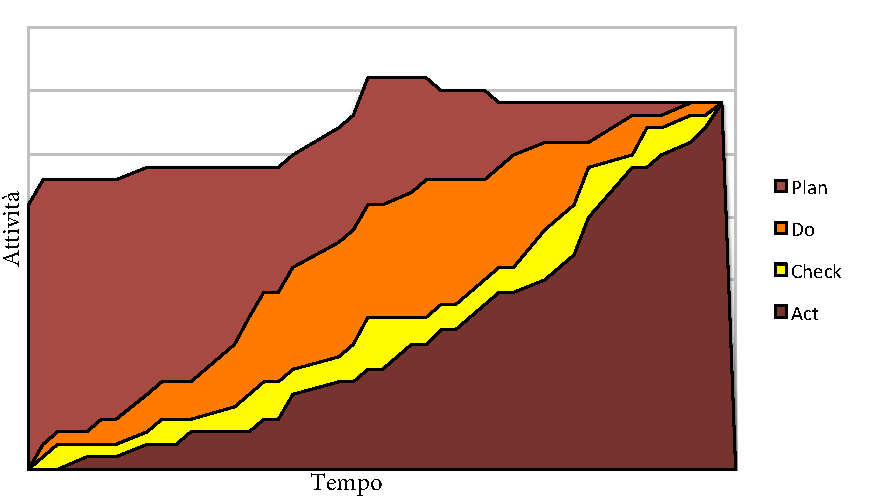
\includegraphics[width=\textwidth]{PianoDiQualifica/Pics/PDCAFaseA.pdf}
							\caption{PDCA Fase A}
						\end{figure}
						Guardando il grafico possiamo notare nella parte centrale un mutamento dei processi pianificati. Le cause di questa mutazione è l'inesperienza pianificazione e dei problemi nella creazione degli Use Case per il documento \insdoc{Analisi dei Requisiti}.\\
						Si può notare inoltre un lieve rallentamento nella parte finale causato dalla vicinanza della sessione di esami e quindi l'aumento degli impegni dei componenti del team.
					\paragraph{Produttività documenti}
						Per le metriche di produttività ed efficacia sulla documentazione si rimanda alla sezione 3.7.3.2 di questo documento.\\
						Sono stati calcolati quindi gli indici di produttività per ogni fase di verifica di ogni documento. A seguito verranno riportate per ogni documento le tabelle con tali valori ed il grafici associati se il periodo di stesura è stato diviso in più fasi incrementali. Fare quindi riferimento al \insdoc{Piano di Progetto}.\\ \\
						Per il documento \insdoc{Norme di Progetto} ho i seguenti valori:				
						\begin{table}[H]\centering
							\begin{tabu}{| l | c |}
								\hline
													&Prima Fase   \\ \hline
												
								Parole scritte				& 3674	 \\ \hline
								Ore Impiegate				& 30	 \\ \hline\hline
							
								Indice di produttività 			 & 122,47 	 \\ \hline
							\end{tabu}
							\caption{Indici di produttività Norme di Progetto}
						\end{table}
						In questo caso non ha senso associare un grafico perché la creazione delle norme di progetto non è stata fatta per incrementi, essendo i tempi di pianificazione stretti e l'impossibilità di scrivere in parallelo altri documenti.\\
					
						Per il documento \insdoc{Studio di Fattibilità} ho i seguenti valori:			
						\begin{table}[H]\centering
							\begin{tabu}{| l | c |}
								\hline
													&Prima Fase   \\ \hline
													
								Parole scritte				& 1507	 \\ \hline
								Ore Impiegate				& 12	 \\ \hline\hline
								
								Indice di produttività 			 & 121,58	  \\ \hline
							\end{tabu}
							\caption{Indici di produttività Studio di Fattibilità}
						\end{table}
						Anche in questo caso è inutile inserire un grafico data la presenza di una singola fase di verifica.\\
					
						Per il documento \insdoc{Analisi dei Requisiti} ho i seguenti valori:	
						\begin{table}[H]\centering
							\begin{tabu}{| l | c | c | c | c |}
								\hline
													&Prima Fase 	& Seconda Fase	& Terza Fase	& Quarta Fase  \\ \hline
												
								Parole scritte				& 730		& 135 		& 3485			& 3288 	 \\ \hline
								Ore Impiegate				& 730		& 135 		& 3485			& 3288 	 \\ \hline\hline
							
								Indice di produttività 			 & 121,67		& 19,29 		& 77,44			& 131,52 	 \\ \hline
							\end{tabu}
							\caption{Indici di produttività Analisi dei Requisiti}
						\end{table}
						Il grafico associato è il seguente:
						\begin{figure}[H]\centering
							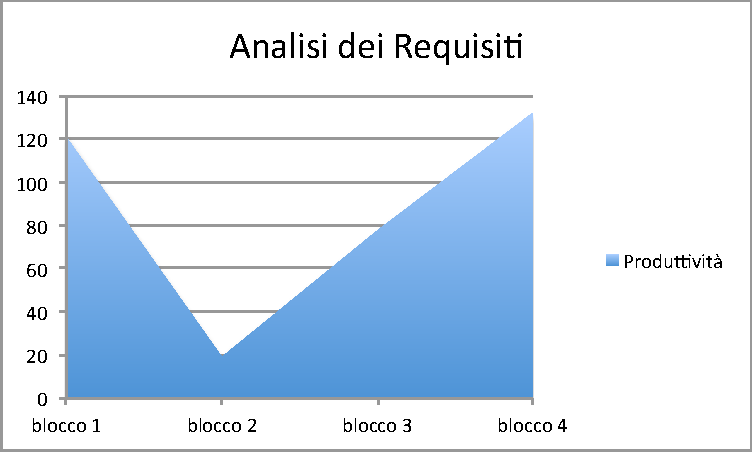
\includegraphics[width=12cm]{PianoDiQualifica/Pics/ProduttivitaAdRFaseA.pdf}
							\caption{Produttività Fase A Analisi dei Requisiti}
						\end{figure}
						In questa fase notiamo un crollo della produttività causato dalla difficoltà riscontrata nella costruzione degli user case dunque alla stesura della loro descrizione e nella stesura dei requisiti.\\
					
						Per il documento \insdoc{Piano di Progetto} ho i seguenti valori:
						\begin{table}[H]\centering
							\begin{tabu}{| X[4] | c | c | c | c | c |}
								\hline
													&Prima Fase 	& Seconda Fase	& Terza Fase	& Quarta Fase 	& Quinta Fase  \\ \hline
												
								Parole scritte				& 1003		& 635 		& 385			& 387 		& 1789 	 \\ \hline
								Ore Impiegate				& 8			& 5 			& 3				& 3	 		& 13	 	  \\ \hline\hline
							
								Indice di produttività 			 & 125,37		& 127 		& 128,33			& 129 		& 137,62 	  \\ \hline
							\end{tabu}
							\caption{Indici di produttività Piano di Progetto}
						\end{table}
						Il grafico associato è il seguente:
						\begin{figure}[H]\centering
							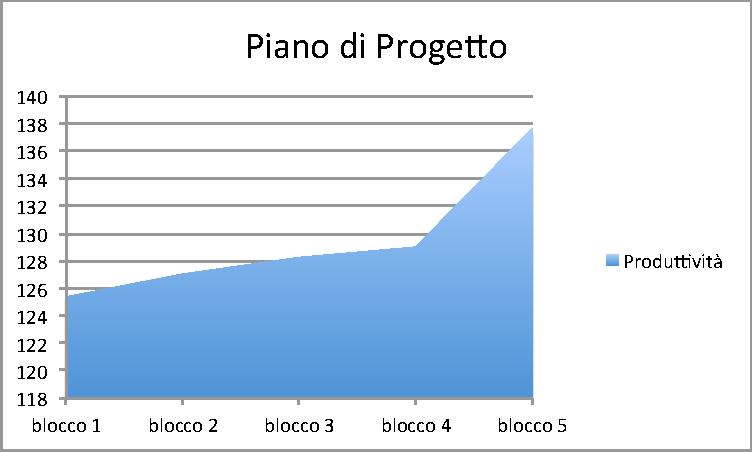
\includegraphics[width=12cm]{PianoDiQualifica/Pics/ProduttivitaPdPFaseA.pdf}
							\caption{Produttività Fase A Piano di Progetto}
						\end{figure}
						Notiamo un miglioramento della produttività, seppur leggero.\\
					
						Per il documento \insdoc{Piano di Qualifica} ho i seguenti valori:	
						\begin{table}[H]\centering
							\begin{tabu}{| l | c | c | c | c |}
								\hline
													&Prima Fase 	& Seconda Fase	& Terza Fase	& Quarta Fase  \\ \hline
												
								Parole scritte				& 378		& 883 		& 760			& 523 	 \\ \hline
								Ore Impiegate				& 3			& 7 			& 6				& 4	 	 \\ \hline\hline
								
								Indice di produttività 			 & 126		& 126,14 		& 126,67			& 130,75 	 \\ \hline
							\end{tabu}
							\caption{Indici di produttività Piano di Qualifica}
						\end{table}
						Il grafico associato è il seguente:
						\begin{figure}[H]\centering
							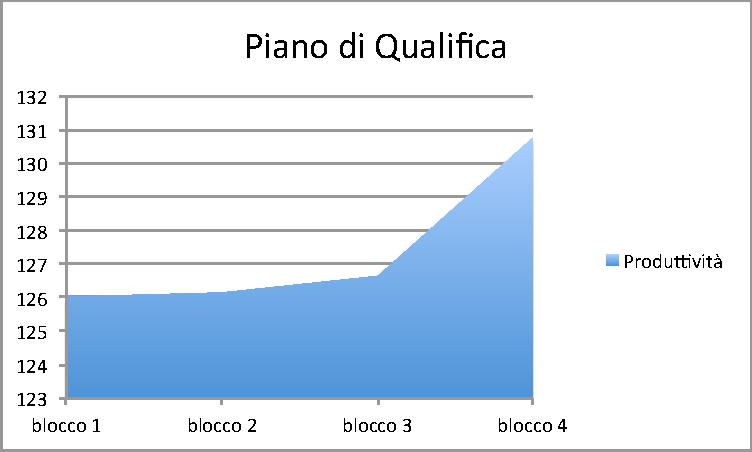
\includegraphics[width=12cm]{PianoDiQualifica/Pics/ProduttivitaPdQFaseA.pdf}
							\caption{Produttività Fase A Piano di Qualifica}
						\end{figure}
						Anche nella stesura di questo documento notiamo gli stessi leggeri miglioramenti avvenuti per il documento precedente.\\
						
						Il grafico seguente rappresenta in ordine cronologico tutti gli indici di produttività calcolati nella fase \insphase{Fase A}.
						\begin{figure}[H]\centering
							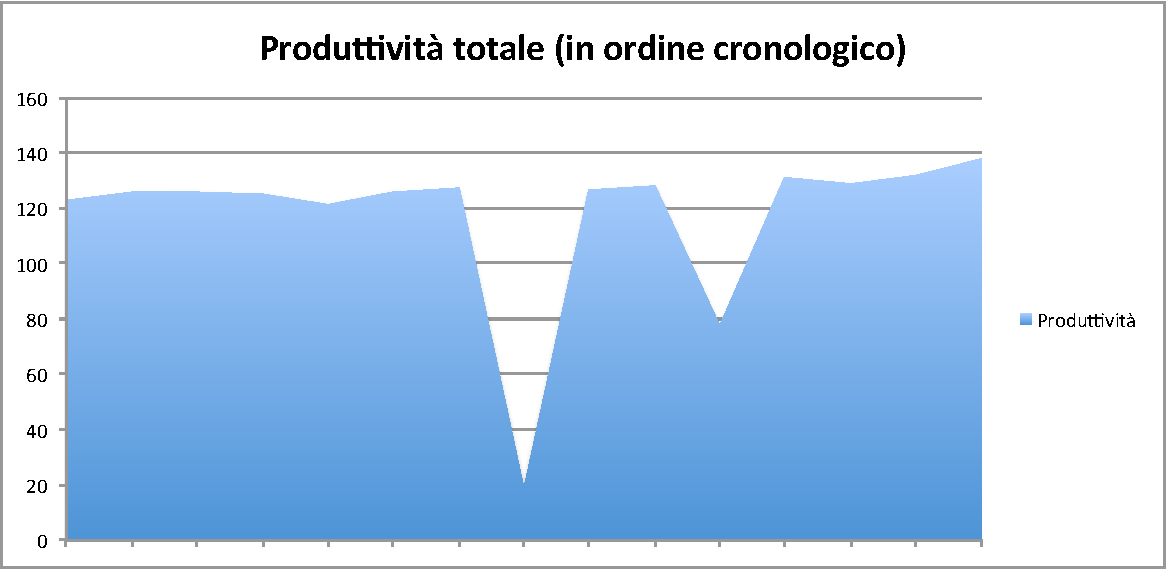
\includegraphics[width=12cm]{PianoDiQualifica/Pics/ProduttivitaTotaleFaseA.pdf}
							\caption{Produttività totale Fase A}
						\end{figure}
						Le cause di questo leggero miglioramento generale sono molto probabilmente le seguenti:
						\begin{itemize}
							\item i componenti del team stanno assimilando le norme di progetto e non devono continuamente far riferimento al documento \insdoc{Norme di Progetto v1.0};
							\item il gruppo sta imparando i comandi \LaTeX{} e di conseguenza la stesura risulta più veloce.
						\end{itemize}						
						Si notano anche i due picchi verso il basso causati dalle iterazioni creatisi nella stesura dell'\insdoc{Analisi dei Requisiti}.
						
					\paragraph{Efficacia della revisione dei documenti}
						Per le metriche di efficacia della revisione sui documenti si rimanda alla sezione 3.7.3.3 di questo documento.\\
						Calcolati questi valori abbiamo quindi quantificato l'efficacia della revisione.
						Sono stati calcolati gli indici di efficacia della revisione per ogni fase di verifica di ogni documento. A seguito verranno riportate per ogni documento le tabelle con tali valori ed il grafici associati se il periodo di stesura è stato diviso in più fasi incrementali. Fare quindi riferimento al \insdoc{Piano di Progetto}.\\ \\
						Per il documento \insdoc{Norme di Progetto} ho i seguenti valori:				
						\begin{table}[H]\centering
							\begin{tabu}{| l | c |}
								\hline
													&Prima Fase   \\ \hline
												
								Errori rilevati				& 311	 \\ \hline
								Pagine ispezionate			& 32		 \\ \hline\hline
							
								Indice di efficacia della revisione 			& 9,72 	 \\ \hline
							\end{tabu}
							\caption{Indici di efficacia della revisione sul documento Norme di Progetto}
						\end{table}
						In questo caso non ha senso associare un grafico per mostrare la variazione di efficacia.
					
						Per il documento \insdoc{Studio di Fattibilità} ho i seguenti valori:			
						\begin{table}[H]\centering
							\begin{tabu}{| l | c |}
								\hline
													&Prima Fase   \\ \hline
												
								Errori rilevati				& 104	 \\ \hline
								Pagine ispezionate			& 11	 \\ \hline\hline
							
								Indice di efficacia della revisione 			 & 9,45	  \\ \hline
							\end{tabu}
							\caption{Indici di efficacia della revisione sul documento Studio di Fattibilità}
						\end{table}
						Anche in questo caso è inutile inserire un grafico data la presenza di una singola fase di verifica.\\
					
						Per il documento \insdoc{Analisi dei Requisiti} ho i seguenti valori:	
						\begin{table}[H]\centering
							\begin{tabu}{| l | c | c | c | c |}
								\hline
													&Prima Fase 	& Seconda Fase	& Terza Fase	& Quarta Fase  \\ \hline
												
								Errori rilevati				& 71		& 12 		& 332			& 234 	 \\ \hline
								Pagine ispezionate			& 7		& 1 		& 30			& 20 	 \\ \hline\hline
							
								Indice di efficacia della revisione 	 & 10,14		& 12 		& 11,07			& 11,7 	 \\ \hline
							\end{tabu}
							\caption{Indici di efficacia della revisione sul documento Analisi dei Requisiti}
						\end{table}
						Il grafico associato è il seguente:
						\begin{figure}[H]\centering
							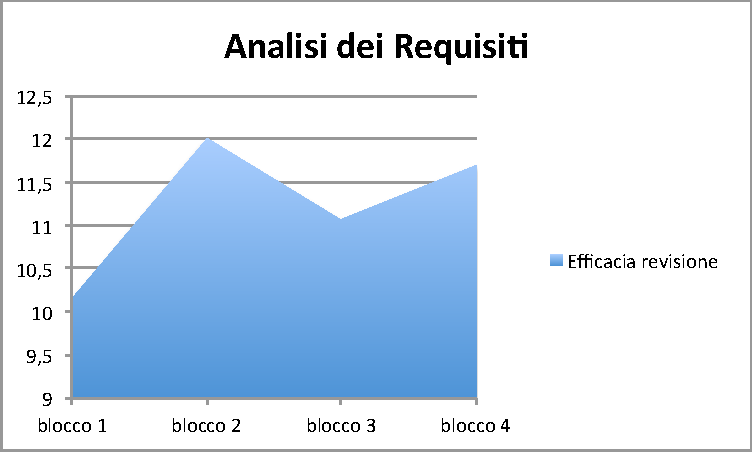
\includegraphics[width=12cm]{PianoDiQualifica/Pics/EfficaciaAdRFaseA.pdf}
							\caption{Efficacia della revisione Fase A Analisi dei Requisiti}
						\end{figure}
						Notiamo un aumento generale dell'efficacia della revisione. Nella seconda fase notiamo un picco verso l'alto semplicemente perchè avendo un numero di pagine bassissimo ogni errore rilevato fa schizzare verso l'alto l'indice di efficacia. Sarebbe quindi un valore da scartare essendo che ci interessa un valore medio.\\
					
						Per il documento \insdoc{Piano di Progetto} ho i seguenti valori:
						\begin{table}[H]\centering
							\begin{tabu}{| X[4] | c | c | c | c | c |}
								\hline
												&Prima Fase 	& Seconda Fase	& Terza Fase	& Quarta Fase 	& Quinta Fase  \\ \hline
												
								Errori rilevati				& 68		& 51 		& 46			& 47 		& 109 	 \\ \hline
								Pagine ispezionate			& 7			& 5 			& 4				& 4	 		& 9	 	  \\ \hline\hline
							
								Indice di efficacia della revisione 	 & 9,71		& 10,2 		& 11,5			& 11,75 		& 12,11 	  \\ \hline
							\end{tabu}
							\caption{Indici di efficacia della revisione sul documento Piano di Progetto}
						\end{table}
						Il grafico associato è il seguente:
						\begin{figure}[H]\centering
							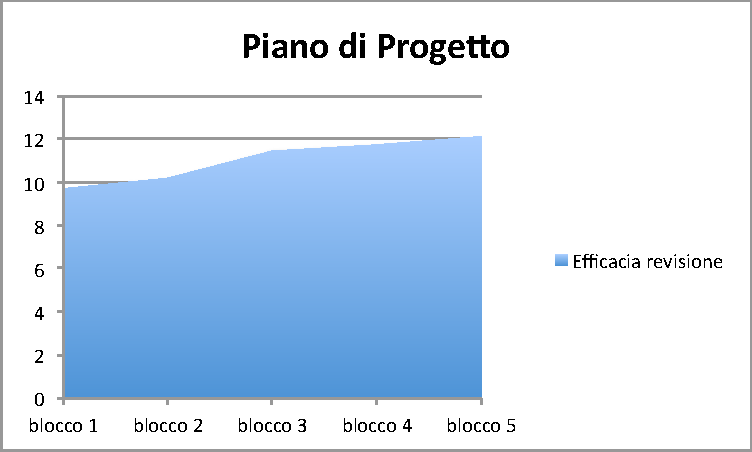
\includegraphics[width=12cm]{PianoDiQualifica/Pics/EfficaciaPdPFaseA.pdf}
							\caption{Efficacia della revisione sul documento Fase A Piano di Progetto}
						\end{figure}
						Notiamo un aumento uniforme dell'efficacia della revisione.
					
						Per il documento \insdoc{Piano di Qualifica} ho i seguenti valori:	
						\begin{table}[H]\centering
							\begin{tabu}{| l | c | c | c | c |}
								\hline
													&Prima Fase 	& Seconda Fase	& Terza Fase	& Quarta Fase  \\ \hline
												
								Errori rilevati				& 27		& 72 		& 60			& 51 	 \\ \hline
								Pagine ispezionate			& 3			& 7 			& 5				& 4	 	 \\ \hline\hline
							
								Indice di efficacia della revisione 	& 9		& 10,29 		& 12			& 12,75 	 \\ \hline
							\end{tabu}
							\caption{Indici di efficacia della revisione sul documento Piano di Qualifica}
						\end{table}
						Il grafico associato è il seguente:
						\begin{figure}[H]\centering
							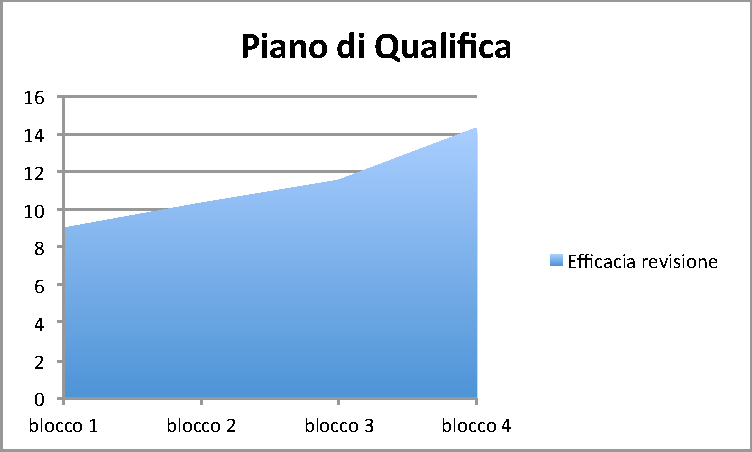
\includegraphics[width=12cm]{PianoDiQualifica/Pics/EfficaciaPdQFaseA.pdf}
							\caption{Efficacia della revisione Fase A Piano di Qualifica}
						\end{figure}
						Anche nella fase di verifica di questo documento notiamo gli stessi miglioramenti avvenuti durante la revisione del documento precedente anche se più accentuati.\\
						
						Il grafico seguente rappresenta in ordine cronologico tutti gli indici di efficacia della revisione calcolati nella fase \insphase{Fase A}.
						\begin{figure}[H]\centering
							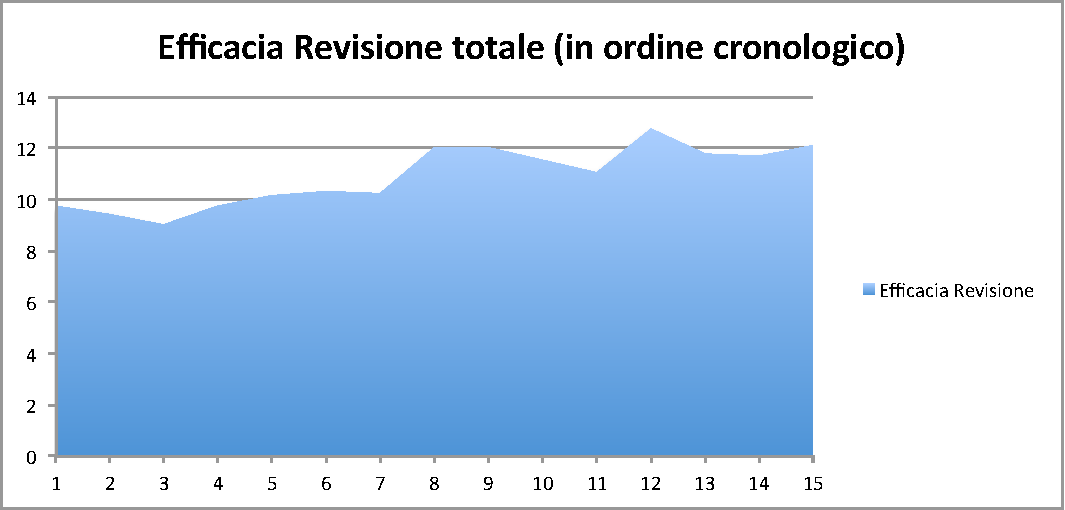
\includegraphics[width=12cm]{PianoDiQualifica/Pics/EfficaciaTotaleFaseA.pdf}
							\caption{Efficacia totale della revisione Fase A}
						\end{figure}
						Questo aumento generale dell'efficacia della revisione è molto probabilmente imputabile all'utilizzo di una lista di controllo (messa in appendice al documento \insdoc{Norme di Progetto}). Si sta infatti cercando di trasformare la fase di verifica da una tecnica walkthrough ad una di tipo inspection rendendoci così più veloci nella ricerca e ciò comporta l'aumento degli errori rilevati.
						
					\paragraph{Produttività casi d'uso}
						Per le metriche di produttività sui casi d'uso si rimanda alla sezione 3.7.3.2 di questo documento.\\
						%TODO
						
						
						 